%\documentclass[mathserif]{beamer}
\documentclass[handout]{beamer}
%\usetheme{Goettingen}
\usetheme{Warsaw}
%\usetheme{Singapore}
%\usetheme{Frankfurt}
%\usetheme{Copenhagen}
%\usetheme{Szeged}
%\usetheme{Montpellier}
%\usetheme{CambridgeUS}
%\usecolortheme{}
%\setbeamercovered{transparent}
\usepackage[english, activeacute]{babel}
\usepackage[utf8]{inputenc}
\usepackage{amsmath, amssymb}
\usepackage{dsfont}
\usepackage{graphics}
\usepackage{cases}
\usepackage{graphicx}
\usepackage{pgf}
\usepackage{epsfig}
\usepackage{amssymb}
\usepackage{multirow}	
\usepackage{amstext}
\usepackage[ruled,vlined,lined]{algorithm2e}
\usepackage{amsmath}
\usepackage{epic}
\usepackage{epsfig}
\usepackage{fontenc}
\usepackage{framed,color}
\usepackage{palatino, url, multicol}
\usepackage{listings}
%\algsetup{indent=2em}
\newcommand{\factorial}{\ensuremath{\mbox{\sc Factorial}}}
\newcommand{\BIGOP}[1]{\mathop{\mathchoice%
{\raise-0.22em\hbox{\huge $#1$}}%
{\raise-0.05em\hbox{\L
\usepackage{fontenc}
\usepackage{framed,color}
\usepackage{palatino, url, multicol}
\usepackage{listings}
%\algsetup{indent=2em}
\newcommand{\factorial}{\ensuremath{\mbox{\sc Factorial}}}
\newcommand{\BIGOP}[1]{\mathop{\mathchoice%
{\raise-0.22em\hbox{\huge $#1$}}%
{\raise-0.05em\hbox{\Large $#1$}}{\hbox{\large $#1$}}{#1}}}
\newcommand{\bigtimes}{\BIGOP{\times}}
\vspace{-0.5cm}
\title{Introduction to Statistical Inference}
\vspace{-0.5cm}
\author[Felipe Bravo Márquez]{\footnotesize
%\author{\footnotesize  
 \textcolor[rgb]{0.00,0.00,1.00}{Felipe José Bravo Márquez}} 
\date{ \today }
arge $#1$}}{\hbox{\large $#1$}}{#1}}}
\newcommand{\bigtimes}{\BIGOP{\times}}
\vspace{-0.5cm}
\title{Introduction to Bayesian Inference}
\vspace{-0.5cm}
\author[Felipe Bravo Márquez]{\footnotesize
%\author{\footnotesize  
 \textcolor[rgb]{0.00,0.00,1.00}{Felipe José Bravo Márquez}} 
\date{ \today }


\begin{document}
\begin{frame}
\titlepage


\end{frame}


%%%%%%%%%%%%%%%%%%%%%%%%%%%


\begin{frame}{Some Critics to the Frequentist Approach}
\scriptsize{
\begin{itemize}
 \item The statistical methods that we have discussed so far are known as frequentist (or classical) methods.
  \item The frequentist approach requires that all probabilities be defined by connection to the frequencies of events in very large samples. 
 \item This leads to frequentist uncertainty being premised on imaginary resampling of data. 
 \item If we were to repeat the measurement many many times, we would end up collecting a list of values that will have some pattern to it. 
 \item  It means also that parameters and models cannot have probability distributions, only measurements can.
 \item The distribution of these measurements is called a sampling distribution. 
 \item This resampling is never done, and in general it doesn't even make sense.
\end{itemize}

} 
\end{frame}

\begin{frame}{Bayesian Inference}
\scriptsize{
There is another approach to inference called Bayesian inference \cite{wasserman2013all}, which is based on the following postulates:
\begin{itemize}
 \item Probability describes \textbf{degree of belief}, not limiting frequency. 
 
 \begin{itemize}
 \scriptsize{
 \item  We can make probability statements about lots of things, not just data which are subject to random variation. 
 \item For example, I might say that "the probability that Albert Einstein drank a cup of tea on August 1, 1948" is .35. 
 \item This does not refer to any limiting frequency. 
 \item It reflects my strength of belief that the proposition is true.}
 \end{itemize}
 
 \item We can make probability statements about parameters, even though they are fixed constants.
 \item We make inferences about a parameter $\theta$ by producing a probability distribution for $\theta$. Inferences, such as point estimates and interval estimates, may then be extracted from this distribution.
\end{itemize}

} 
\end{frame}


\begin{frame}{Bayesian Inference}
\scriptsize{
\begin{itemize}
 \item In modest terms, Bayesian data analysis is no more than counting the numbers of ways
the data could happen, according to our assumptions \cite{mcelreath2020statistical}.
 \item In Bayesian analysis all alternative sequences of events that could have generated our data are evaluated.
 \item As we learn about what did happen, some of these alternative sequences are pruned. 
 \item In the end, what remains is only what is logically consistent with our knowledge \cite{mcelreath2020statistical}.
 \item Warning: understanding the essence of Bayesian inference can be hard.
 \item The following toy example tries to explain it in a gentle way.
\end{itemize}
 } 
\end{frame}


\begin{frame}{Counting Possibilities}
\scriptsize{
\begin{itemize}
 \item Suppose there's a bag, and it contains \textbf{four} marbles.
 \item These marbles come in two colors: \textbf{blue} and \textbf{white}. 
 \item We know there are four marbles in the bag, but we don't know how many are of each color. 
 \item We do know that there are five possibilities: 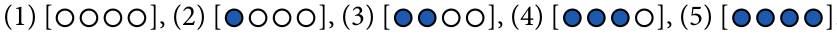
\includegraphics[scale=0.3]{pics/marbles1.png}
 \item These are the only possibilities consistent with what we know about the contents of the bag. Call these five possibilities the \textbf{conjectures}.
 \item Our goal is to figure out which of these conjectures is most \textbf{plausible}, given some \textbf{evidence} about the contents of the bag. 
 \item Evidence: A sequence of three marbles is pulled from the bag, one at a time, replacing the marble each time and shaking the bag, in that order. 
 \item The sequence that emerges is: 
\includegraphics[scale=0.5]{pics/marbles2.png}, which is our \textbf{data}. 
  
\end{itemize}
 } 
\end{frame}



\begin{frame}{Counting Possibilities}
\scriptsize{
\begin{itemize}
 \item Now, let's see how to use the data to infer what's in the bag.
 \item Let's begin by considering just the single conjecture, 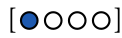
\includegraphics[scale=0.3]{pics/marbles3.png}, that the bag contains one blue and three white marbles. 
 \item On the first draw from the bag, one of four things could
happen, corresponding to one of four marbles in the bag.

\begin{figure}[h!]
	\centering
	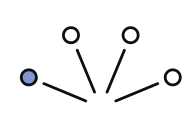
\includegraphics[scale=0.4]{pics/marbles4.png}
\end{figure}

\item Notice that even though the three white marbles look the same from a data perspective we just record the color of the marbles, after all they are really different events.

\item This is important, because it means that there are three more ways to see 
\includegraphics[scale=0.3]{pics/marbles5.png} than to see 
\includegraphics[scale=0.3]{pics/marbles6.png}.

\end{itemize}
 } 
\end{frame}



\begin{frame}{Counting Possibilities}
\scriptsize{
\begin{itemize}
 \item Now consider the garden as we get another draw from the bag. It expands the garden out one layer:

\begin{figure}[h!]
	\centering
	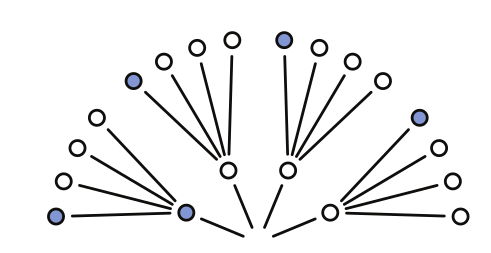
\includegraphics[scale=0.4]{pics/marbles7.png}
\end{figure}

\item Now there are 16 possible paths through the garden, one for each pair of draws.

\item On the second draw from the bag, each of the paths above again forks into four possible paths. Why?

\end{itemize}
 } 
\end{frame}


\begin{frame}{Counting Possibilities}
\scriptsize{
\begin{itemize}
 \item Because we believe that our shaking of the bag gives each marble a fair chance at being drawn, regardless of which marble was drawn previously. \item The third layer is built in the same way, and the full garden is shown
 below:
\begin{figure}[h!]
	\centering
	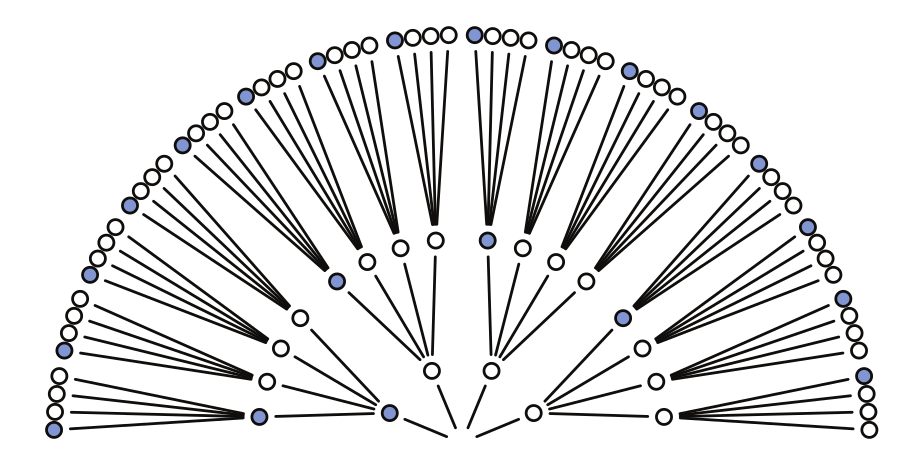
\includegraphics[scale=0.3]{pics/marbles8.png}
\end{figure}

\item There are $4^3 = 64$ possible paths in total.

\end{itemize}
 } 
\end{frame}


\begin{frame}{Counting Possibilities}
\scriptsize{
\begin{itemize}
 \item As we consider each draw from the bag to get 
\includegraphics[scale=0.5]{pics/marbles2.png}, some of these paths are logically eliminated.
 \item The first draw tuned out to be 
\includegraphics[scale=0.3]{pics/marbles6.png}, recall, so the three white paths at the bottom are eliminated right away. 
 \item If you imagine the real data tracing out a path, it must have passed through the one blue path near the origin. 
 \item The second draw from the bag produces 
\includegraphics[scale=0.3]{pics/marbles5.png}, so three of the paths forking out of the first blue marble remain.
 \end{itemize}
 } 
\end{frame}


\begin{frame}{Counting Possibilities}
\scriptsize{
\begin{itemize}
 \item As the data trace out a path, we know it must have passed through one of those three white paths (after the first blue path).
 \item But we don't know which one, because we recorded only the color of each marble.
 \item Finally, the third draw is 
\includegraphics[scale=0.3]{pics/marbles6.png}. 
 \item Each of the remaining three paths in the middle layer sustain one blue path, leaving a total of three ways for the sequence 
\includegraphics[scale=0.3]{pics/marbles2.png} to appear, assuming the bag contains 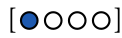
\includegraphics[scale=0.3]{pics/marbles3.png}.
\end{itemize}
 } 
\end{frame}


\begin{frame}{Counting Possibilities}
\scriptsize{
\begin{itemize}
 \item The figure below shows the forking paths again, now with logically eliminated paths grayed out.

\begin{figure}[h!]
	\centering
	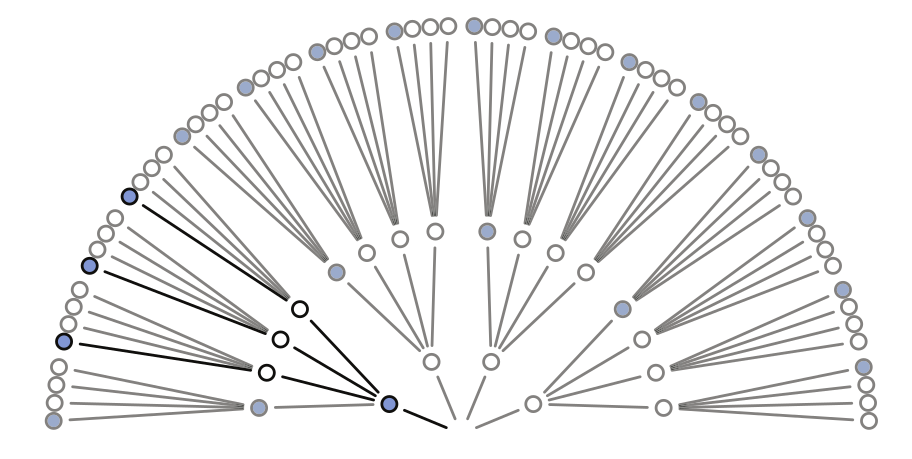
\includegraphics[scale=0.33]{pics/marbles9.png}
\end{figure}
\end{itemize}
 } 
\end{frame}



\begin{frame}{Counting Possibilities}
\scriptsize{
\begin{itemize}
\item We can't be sure which of those three paths the actual data took.
\item But as long as we're considering only the possibility that the bag contains one blue and three white marbles, we can be sure that the data took one of those three paths.

\item Those are the only paths consistent with both our knowledge of the bag's contents (four marbles, white or blue) and the data (
\includegraphics[scale=0.3]{pics/marbles2.png}).  

 \item This demonstrates that there are three (out of 64) ways for a bag containing to produce the data.
 \item We have no way to decide among these three ways. 
\end{itemize}
 } 
\end{frame}


\begin{frame}{Counting Possibilities}
\scriptsize{
\begin{itemize}
 \item The inferential power comes from comparing this count to the numbers of ways each of the other conjectures of the bag's contents could produce the same data. 
 \item For example, consider the conjecture 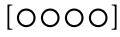
\includegraphics[scale=0.3]{pics/marbles10.png}. 
 \item There are zero ways for this conjecture to produce the observed data, because even one 
\includegraphics[scale=0.3]{pics/marbles6.png} is logically incompatible with it. 
\item The conjecture 
\includegraphics[scale=0.3]{pics/marbles11.png} is likewise logically incompatible with the data. 
\item So we can eliminate these two conjectures, because neither provides even a single path that is consistent with the data.
\item The next slide's figure displays all the paths for the reamaining three conjectures: 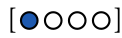
\includegraphics[scale=0.3]{pics/marbles3.png}, 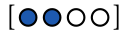
\includegraphics[scale=0.3]{pics/marbles13.png}, and 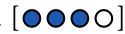
\includegraphics[scale=0.3]{pics/marbles14.png}.

\end{itemize}
 } 
\end{frame}




\begin{frame}{Counting Possibilities}
\scriptsize{
\begin{figure}[h!]
	\centering
	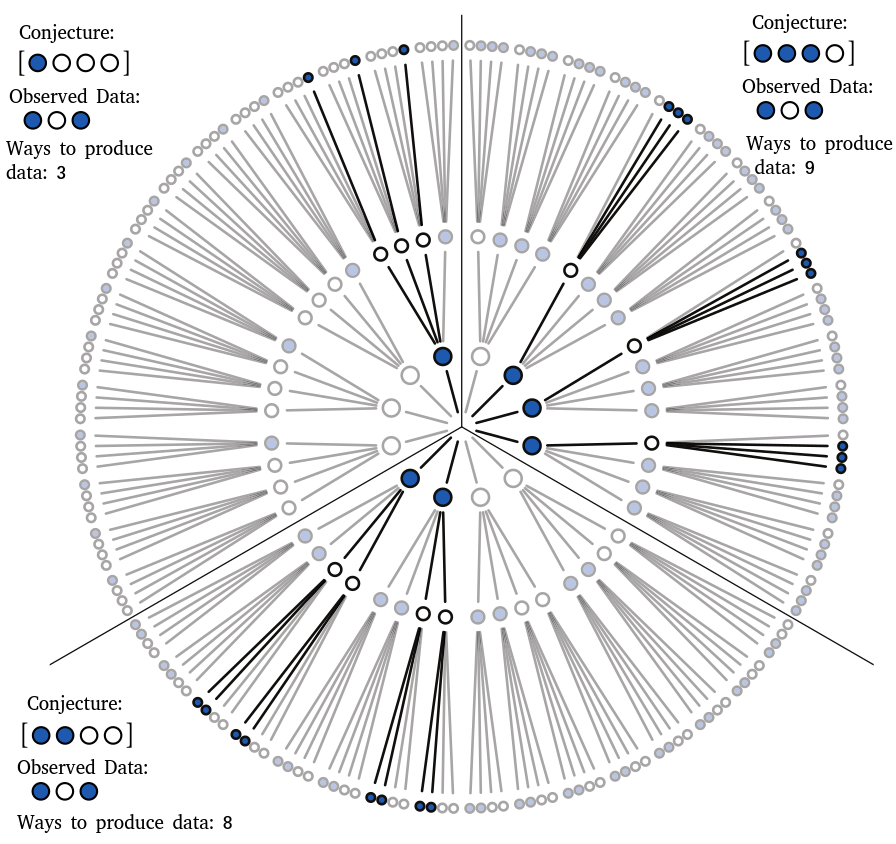
\includegraphics[scale=0.35]{pics/marbles12.png}
\end{figure}
 } 
\end{frame}

\begin{frame}{Counting Possibilities}
\scriptsize{
\begin{itemize}
 \item The number of ways to produce the data, for each conjecture, can be computed by first counting the number of paths in each ``ring'' of the garden and then by multiplying these counts together.
 \begin{figure}[h!]
	\centering
	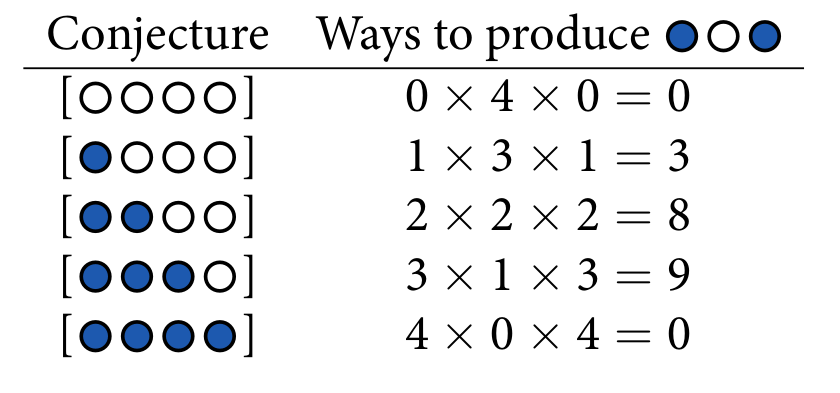
\includegraphics[scale=0.3]{pics/marbles15.png}
\end{figure}
\item By comparing these counts, we have part a way to rate the relative \textbf{plausibility} of each conjectured bag composition.
\end{itemize}
 } 
\end{frame}

\begin{frame}{Combining other information}
\scriptsize{
\begin{itemize}
 \item We may have additional information about the relative plausibility of each conjecture. 
 \item This information could arise from knowledge of how the contents of the bag were generated. 
 \item It could also arise from previous data. 
 \item Whatever the source, it would help to have a way to combine different sources of information to update the plausibilities. 
 \item Luckily there is a natural solution: Just multiply the counts.
\end{itemize}
 } 
\end{frame}


\begin{frame}{Combining other information}
\scriptsize{
\begin{itemize}
 \item Suppose that each conjecture is equally plausible at the start.
 \item So we just compare the counts of ways in which each conjecture is compatible with the observed data: 
\includegraphics[scale=0.3]{pics/marbles2.png}.
 \item This comparison suggests that 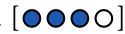
\includegraphics[scale=0.3]{pics/marbles14.png} is slightly more plausible than 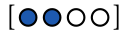
\includegraphics[scale=0.3]{pics/marbles13.png}, and both are about three times more plausible than 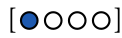
\includegraphics[scale=0.3]{pics/marbles3.png}. 
\item Since these are our initial counts, and we are going to update them next, let's label them \textbf{prior}.
\item Now suppose we draw another marble from the bag to get another observation: 
\includegraphics[scale=0.3]{pics/marbles6.png}. 
\item How can we update our plausibilities about each conjecture based on this new evidence?
\item There are two choices discussed next. 
\end{itemize}
 } 
\end{frame}


\begin{frame}{Combining other information}
\scriptsize{
\begin{itemize}
 \item Option 1: draw a forking path with four layers and do the counting again.
\item Option 2: Update previous counts (0, 3, 8, 9, 0) with the new information by multiplying the new count by the old count.
\item Both approach are matematically identical as long
as the new observation is logically independent of the previous observations. 

\begin{figure}[h!]
	\centering
	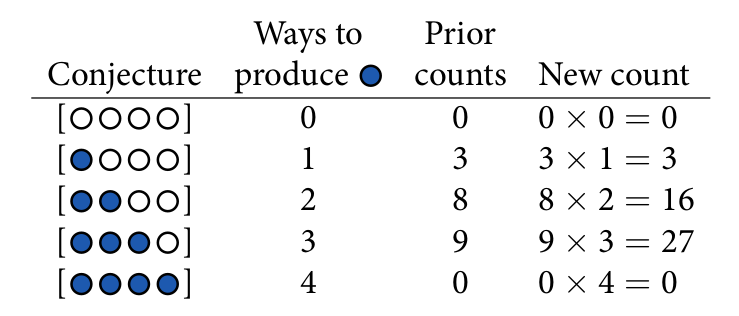
\includegraphics[scale=0.33]{pics/marbles16.png}
\end{figure}
\end{itemize}
 } 
\end{frame}



\begin{frame}{Combining other information}
\scriptsize{
\begin{itemize}
 \item In the previous example, the prior data and new data are of the same type: marbles drawn from the bag. 
 \item But in general, the prior data and new data can be of different types. 
 \item Suppose for example that someone from the marble factory tells you that blue marbles are rare.
 \item So for every bag containing 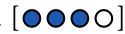
\includegraphics[scale=0.3]{pics/marbles14.png}, they made two bags containing 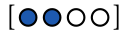
\includegraphics[scale=0.3]{pics/marbles13.png} and three bags containing 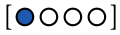
\includegraphics[scale=0.3]{pics/marbles17.png} . 
 \item They also ensured that every bag contained at least one blue and one white marble. 
\end{itemize}
 } 
\end{frame}


\begin{frame}{Combining other information}
\scriptsize{
\begin{itemize}
 \item We can update our counts again:
\begin{figure}[h!]
	\centering
	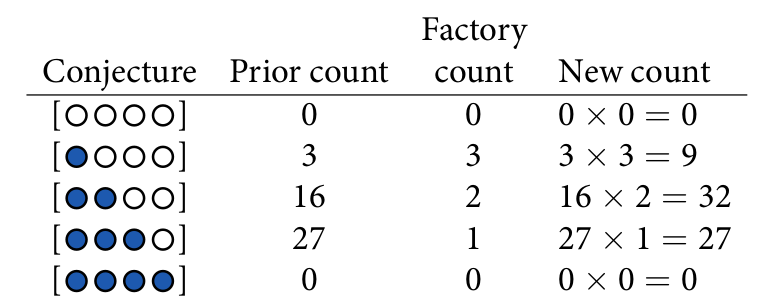
\includegraphics[scale=0.33]{pics/marbles18.png}
\end{figure}
\item Now the conjecture 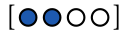
\includegraphics[scale=0.3]{pics/marbles13.png} is most plausible, but barely better than 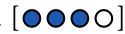
\includegraphics[scale=0.3]{pics/marbles14.png}.
\item Is there a threshold difference in these counts at which we can safely decide that one of the conjectures is the correct one? 
\item We will explore this question next.
\end{itemize}
 } 
\end{frame}

\begin{frame}{From counts to probability}
\scriptsize{
\begin{itemize}
 \item  So far, we have defined the updated plausibility of each possible composition of the bag, after seeing the data, as:
 \begin{figure}[h!]
	\centering
	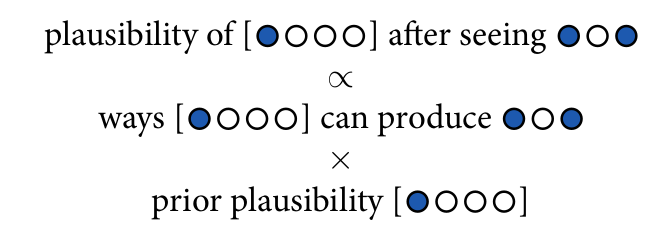
\includegraphics[scale=0.3]{pics/marbles19.png}
\end{figure}
\item The problem of representing plausibilities as counts is that these numbers grow very quickly  as  the amount of data grows. 
 \item It is better to standardize them to turn them into probabilities.
\end{itemize}
 } 
\end{frame}


\begin{frame}{From counts to probability}
\scriptsize{
\begin{itemize}
 \item Now  we will formalize the Bayesian framework using probabilities.
\item Let index our conjecture with a parameter $\theta$ defined as the fractions of marbles from the bag that are blue:

$\theta=0 \rightarrow$ 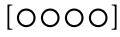
\includegraphics[scale=0.3]{pics/marbles10.png}, $\theta=0.25 \rightarrow$ 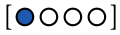
\includegraphics[scale=0.3]{pics/marbles17.png}, $\theta=0.5 \rightarrow$ 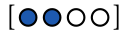
\includegraphics[scale=0.3]{pics/marbles13.png},  $\theta=0.75 \rightarrow$ 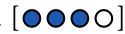
\includegraphics[scale=0.3]{pics/marbles14.png}, $\theta=1 \rightarrow$ 
\includegraphics[scale=0.3]{pics/marbles11.png}.

\item Let's call our data 
\includegraphics[scale=0.3]{pics/marbles2.png} $d$. 

\item We construct probabilities by standardizing the plausibility so that the sum of the plausibilities for all possible conjectures will be one.

\begin{equation}
 \text{plausibility of $\theta$ after $d$} = \frac{\text{ways $\theta$ can produce $d$} \times \text{prior plausibility $\theta$}}{\text{sum of products}}
\end{equation}

\item This is essentially the Bayes theorem:

\begin{equation}
 \mathbb{P}(\theta|d) = \frac{\mathbb{P}(d|\theta) \times \mathbb{P}(\theta)}{\mathbb{P}(d)}
\end{equation}


\end{itemize}
 } 
 
 \end{frame}



\begin{frame}{From counts to probability}
\scriptsize{
\begin{itemize}
\item The denominator $\mathbb{P}(d)$ (that standardizes values to sum one) can be expressed by the law of total probabilities as: 
\begin{equation}
 \mathbb{P}(d) =  \sum_\theta \mathbb{P}(d|\theta) \times \mathbb{P}(\theta) 
\end{equation}

 \item Let's consider the prior assumptions that all conjectures are equally plausible at the start, then $\mathbb{P}(\theta)$ is uniformly distributed.  \\ 
 
 \vspace{0.3cm}
  \begin{tabular}{c|c|c|c|c} \hline
$\theta$ & $\mathbb{P}(\theta)$ & Ways to Produce Data & $\mathbb{P}(d|\theta)$ & $\mathbb{P}(\theta|d) = \mathbb{P}(d|\theta)*\mathbb{P}(\theta) / \mathbb{P}(d)$  \\ \hline
0 & 1/5 & 0 & 0/64 &  $\frac{0/64*1/5}{0.0625}$ =0 \\
0.25 & 1/5 & 3 & 3/64 & $\frac{3/64*1/5}{0.0625}$ = 0.15
\\
0.5 & 1/5 & 8 & 8/64 & $\frac{8/64*1/5}{0.0625}$ = 0.4 \\
0.75 & 1/5 & 9 & 9/64 & $\frac{9/64*1/5}{0.0625}$ = 0.45 \\
1 & 1/5 & 0 & 0/64 & $\frac{0/64*1/5}{0.0625}$ = 0 \\ 
\end{tabular} 
\vspace{0.3cm} 
 
\item where $\mathbb{P}(d)$ = 1/5 * 0/64 + 1/5*3/64 + 1/5*8/64+1/5*9/64+1/5*0/64 = 0.0625 
 
 
\end{itemize}
 } 
 

\end{frame}


\begin{frame}{From counts to probability}
\scriptsize{
\begin{itemize}
\item Let's use the factory counts information (blue marbles are rare) now in our prior assumptions of $\mathbb{P}(\theta)$.  \\ 
\item This can be done by normalizing the factory counts.  

\item Notice that this new prior assumption doesn't affect the ways each conjecture can generate the data and $\mathbb{P}(d|\theta)$ remains unchanged.
 
 \vspace{0.3cm}
  \begin{tabular}{c|c|c|c|c} \hline
$\theta$ & Factory count & $\mathbb{P}(\theta)$ &  $\mathbb{P}(d|\theta)$ & $\mathbb{P}(\theta|d) = \mathbb{P}(d|\theta)*\mathbb{P}(\theta) / \mathbb{P}(d)$  \\ \hline
0 & 0 & 0/6 &  0/64 &  $\frac{0/64*0/6}{0.08854167}$ =0 \\
0.25 & 3 & 3/6 & 3/64 & $\frac{3/64*3/6}{0.08854167}$ = 0.2647059
\\
0.5 & 2 & 2/6  & 8/64 & $\frac{8/64*2/6}{0.08854167}$ = 0.4705882 \\
0.75 & 1 &  1/6 & 9/64 & $\frac{9/64*1/6}{0.08854167}$ = 0.2647059  \\
1 &  0 & 0/6 &  0/64 & $\frac{0/64*0/6}{0.08854167}$ = 0 \\ 
\end{tabular} 
\vspace{0.3cm} 
 
\item where $\mathbb{P}(d)$= 0/6 * 0/64 + 3/6*3/64 + 2/6*8/64+1/6*9/64+0/6*0/64 =  0.08854167

\item Two different prior assumptions led us to different values of $\mathbb{P}(\theta|d)$.
 
\end{itemize}
 } 

\end{frame}


\begin{frame}{From counts to probability}
\scriptsize{
\begin{figure}[h!]
	\centering
	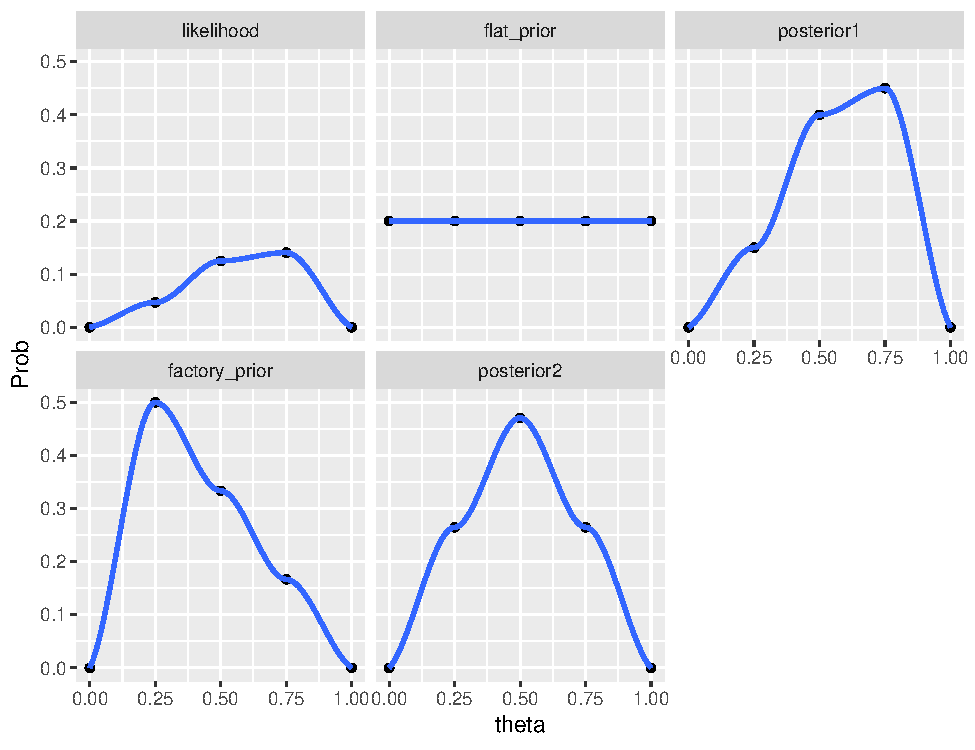
\includegraphics[scale=0.63]{pics/marbles_dist.pdf}
\end{figure}
 } 
 

\end{frame}


\begin{frame}{Bayesian Components}
\scriptsize{
Now we will introduce the names of the components of our Bayesian model. 

\begin{itemize}
\item \textbf{Parameter} $\theta$:  A way of indexing possible explanations of the data. In our example is a conjectured proportion of blue marbles. 

\item \textbf{Likelihood} $\mathbb{P}(d|\theta)$: The relative number of ways that a value $\theta$ can produce the data. It is derived by enumerating all the possible data sequences that could have happened and then eliminating those sequences inconsistent with the data.
\item \textbf{Prior probability} $\mathbb{P}(\theta)$: The prior plausibility of any specific value of $\theta$.
 
\item \textbf{Posterior probability} $\mathbb{P}(\theta|d)$: The new, updated plausibility of any specific $\theta$. 

\item \textbf{Evidence} or \textbf{Average Likelihood} $\mathbb{P}(d)$: the average probability of the data averaged over the prior. It’s job is just to standardize the posterior, to ensure it sums (integrates) to one. 
 
\end{itemize}
 } 

All these components are connected by the Bayes theorem!
 
\end{frame}


\begin{frame}{Bayesian Components}
\scriptsize{
\begin{itemize}

\item It is important to remark that in the Bayesian setting a parameter $\theta$ is random a variable, so we can make probability staments about it.

\item Whereas in the frequentist approach parameters are considered unknown quantities. 

\item This is an important property of Bayesian inference: despite $\theta$ is an \textbf{unobseved variable} we can treat is a random variable and calculate $\mathbb{P}(\theta)$ or $\mathbb{P}(\theta|d)$.

\item The likelihood function  $\mathbb{P}(d|\theta)$ is very similar to the likelihood function in the frequentist approach $\mathbb{P}(d;\theta)$ but now we can condition of $\theta$ instead of just using it as function parameter.

\item All the probability functions of a Bayesian model can correspond to either 1) a probability mass or 2) a density functions depending if the variable (observed or unobserved) are discrete or continous.


\end{itemize}
 } 

\end{frame}


\begin{frame}{Bayesian Components}
\scriptsize{
\begin{itemize}

\item In the marble example $\theta$ is discrete so the prior and the posterior are probability mass functions.

\item When $\theta$ is continous, the \textbf{evidence} is calculated with an integral called \textbf{marginal}

\begin{equation}
 \mathbb{P}(d) = \int_{\theta}\mathbb{P}(d|\theta)\mathbb{P}(\theta)d\theta  
\end{equation}

\item In most cases this integral doesn't have a closed solution.

\item But there some nice computational methods available that can efficiently approximate the posterior. 

\item Next, we will go deeper into these concepts by building another Bayesian toy model.
 
\end{itemize}
 } 

\end{frame}



\begin{frame}{A Globe Model}
\scriptsize{
\begin{itemize}

\item We have a globe representing our planet. 
\item We want to estimate much of the surface is covered in water. 
\item We adopt the following strategy: we toss the globe up in the air, we catch it, record whether or not the surface under your right index finger is water or
land. 
\item Then we toss the globe up in the air again and repeat the procedure.
\item The first nine samples are:
W L W W W L W L W
where W indicates water and L indicates land.
\item We observed 6 W and 3 L. This is our data.
\end{itemize}
 } 
 
\scriptsize{
\begin{figure}[h!]
	\centering
	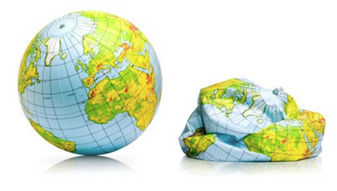
\includegraphics[scale=0.4]{pics/globe.png}
\end{figure}
 }  

\end{frame}

\begin{frame}{A Globe Model}
Designing a simple Bayesian model benefits from a design loop with three steps.
\begin{enumerate}
 \item Data story: Motivate the model by narrating how the data might arise.
\item Update: Educate your model by feeding it the data.
\item Evaluate: All statistical models require supervision, leading to model revision.
\end{enumerate}

\end{frame}



\begin{frame}{A Globe Model}
\scriptsize{
\begin{itemize}

\item Bayesian data analysis usually means producing a story for how the data came to be.
\item This story may be descriptive, specifying associations that can be used to predict outcomes, given observations. 
\item Or it may be causal, a theory of how some events
produce other events.
\item You can motivate your data story by trying to explain how each piece of data is born. 
\item This usually means describing aspects of the underlying reality as well as the sampling process.
\end{itemize}
 } 
\end{frame}

\begin{frame}{A Globe Model}
\scriptsize{
\begin{itemize}
\item You can motivate your data story by trying to explain how each piece of data is born. 
\item This usually means describing aspects of the underlying reality as well as the sampling process.
\item The data story in this case is simply a restatement of the sampling process:

\begin{enumerate}
\scriptsize{
 \item The true proportion of water covering the globe is $p$.
 \item A single toss of the globe has a probability $p$ of producing W and $1-p$ of producing L.
\item Each toss of the globe is independent of the others.}
\end{enumerate}

\item The data story is then translated into a formal probability model where we assign distributions to our Bayesian components.
\end{itemize}




} 
 
 

\end{frame}



%%%%%%%%%%%%%%%%%%%%%%%%%%%
\begin{frame}[allowframebreaks]\scriptsize
\frametitle{References}
\bibliography{bio}
\bibliographystyle{apalike}
%\bibliographystyle{flexbib}
\end{frame}  









%%%%%%%%%%%%%%%%%%%%%%%%%%%

\end{document}
